\documentclass{tietreport}

% Import packages
\usepackage{graphicx}
\graphicspath{{images/}}
\usepackage{booktabs}
\usepackage{listings}
\usepackage{xcolor}

% Bibliography configuration
\usepackage[
  date=year,
  style=alphabetic,
  backend=biber,
  sorting=nty,
  maxnames=5,
  minnames=3,
  maxalphanames=4,
  minalphanames=3,
  backref=true,
  doi=false,
  isbn=false,
  url=false,
  eprint=false
]{biblatex}
\addbibresource{references.bib}

%% ==================================================
%% CUSTOMIZE FIELDS FOR CIVICSCAN PROJECT
%% ==================================================

\TitlePageHeader{%
  UCS503P - Software Engineering Project Report%
}

\ProjectTitle{%
  CivicScan: AI-Based Civic\\ Problem Reporter%
}

\ProjectSubTitle{%
  Smart City Issue Detection, Severity Estimation\\ \& Department Routing%
}

\author{%
  \texttt{1024030806} Chintan Sood \\
  \texttt{1024030807} Tanu Bansal \\
  \texttt{1024030802} Adhyan Gupta%
}

\TitlePageSubText{%
  Group: BE Third Year, CSE%
}

\AdvisorName{%
  Dr. Nisha Thakur%
}

\TitlePageFooterText{{%
    \large Mid-Semester Evaluation \\[0.2cm]
    \bfseries Computer Science and Engineering Department%
  } \\[0.15cm]
  Thapar Institute of Engineering and Technology, Patiala%
}

%% ==================================================

\begin{document}

% Generate title page
\maketitle

% Table of contents
\tableofcontents

% ===== CHAPTER 1: INTRODUCTION =====

\chapter{Introduction}

\section{Background and Context}

Urban India is experiencing rapid urbanization, leading to an increasing burden on municipal civic infrastructure. Potholes, overflowing garbage dumps, damaged sidewalks, and urban waterlogging pose safety hazards and reduce the quality of life for citizens. Currently, municipal grievance reporting in many Indian cities relies on fragmented manual channels, such as paper forms, helpline phone calls, and social media posts~\cite{whent2022civic}. These existing workflows lack automated issue categorization, severity quantification, and real-time status tracking for citizens.

\subsection{Problem Statement}

Citizens face several challenges when reporting municipal issues:
\begin{itemize}
  \item \textbf{Manual Categorization:} Citizens are required to self-identify complex issue categories, leading to mislabeled reports and administrative rework.
  \item \textbf{Absence of Severity Signals:} Reports are treated with uniform priority regardless of hazard severity, making prioritization subjective.
  \item \textbf{Opaque Routing:} Manual inbox processing delays issue dispatching to specialized municipal departments (e.g., Sanitation vs. Roads Department).
  \item \textbf{Lack of Transparency:} Citizens have minimal visibility into report progression after submission.
\end{itemize}

CivicScan addresses these challenges by delivering an end-to-end AI-powered web platform that automates civic problem detection, computes objective severity scores, captures precise GPS coordinates, and plots live active reports on a city map.

\section{Project Objectives}

The primary objectives of the CivicScan project for Module 1 are:

\begin{enumerate}
  \item \textbf{Objective 1 (Computer Vision Pipeline):} Fine-tune a YOLOv8 object detection model to identify municipal infrastructure issues (road damage, garbage accumulation, waterlogging) from citizen photo uploads with an mAP50 target $\ge 0.70$~\cite{ultralytics2023yolov8}.
  \item \textbf{Objective 2 (Automated Severity Calculation):} Implement a deterministic mathematical model combining detection confidence and bounding box area ratio to calculate issue severity (Low, Medium, High).
  \item \textbf{Objective 3 (Full-Stack Core Functionality):} Build a responsive Next.js frontend integrated with a FastAPI backend, client-side HTML5 Geolocation API, and interactive live map pin plotting~\cite{fastapi2024, nextjs2024}.
\end{enumerate}


% ===== CHAPTER 2: METHODOLOGY & DESIGN =====

\chapter{Methodology and Design}

\section{System Architecture}

CivicScan follows a modular microservice-style full-stack web architecture separating the user presentation layer, API routing, and AI computer vision inference.

\subsection{High-Level Design}

The system flow consists of three primary layers for core functionality:
\begin{enumerate}
  \item \textbf{Presentation Layer (Next.js):} Provides the Citizen Portal for uploading photos, capturing GPS coordinates, and rendering a dynamic Leaflet-style live map with interactive issue pins.
  \item \textbf{API \& Business Logic Layer (FastAPI):} Serves RESTful detection endpoints (\texttt{/detect}, \texttt{/submit-report}), handles CORS middleware, and formats location coordinates.
  \item \textbf{AI Machine Learning Layer (Ultralytics YOLOv8):} Executes real-time object detection on input images, generates annotated bounding box overlays, and returns detection metadata alongside Base64 encoded result images~\cite{ramalingam2021smartcity}.
\end{enumerate}

\subsection{System Diagrams \& Workflow Models}

To visually model system actor interactions and cross-component control flow, the architecture includes structural UML models:

\begin{figure}[h!]
  \centering
  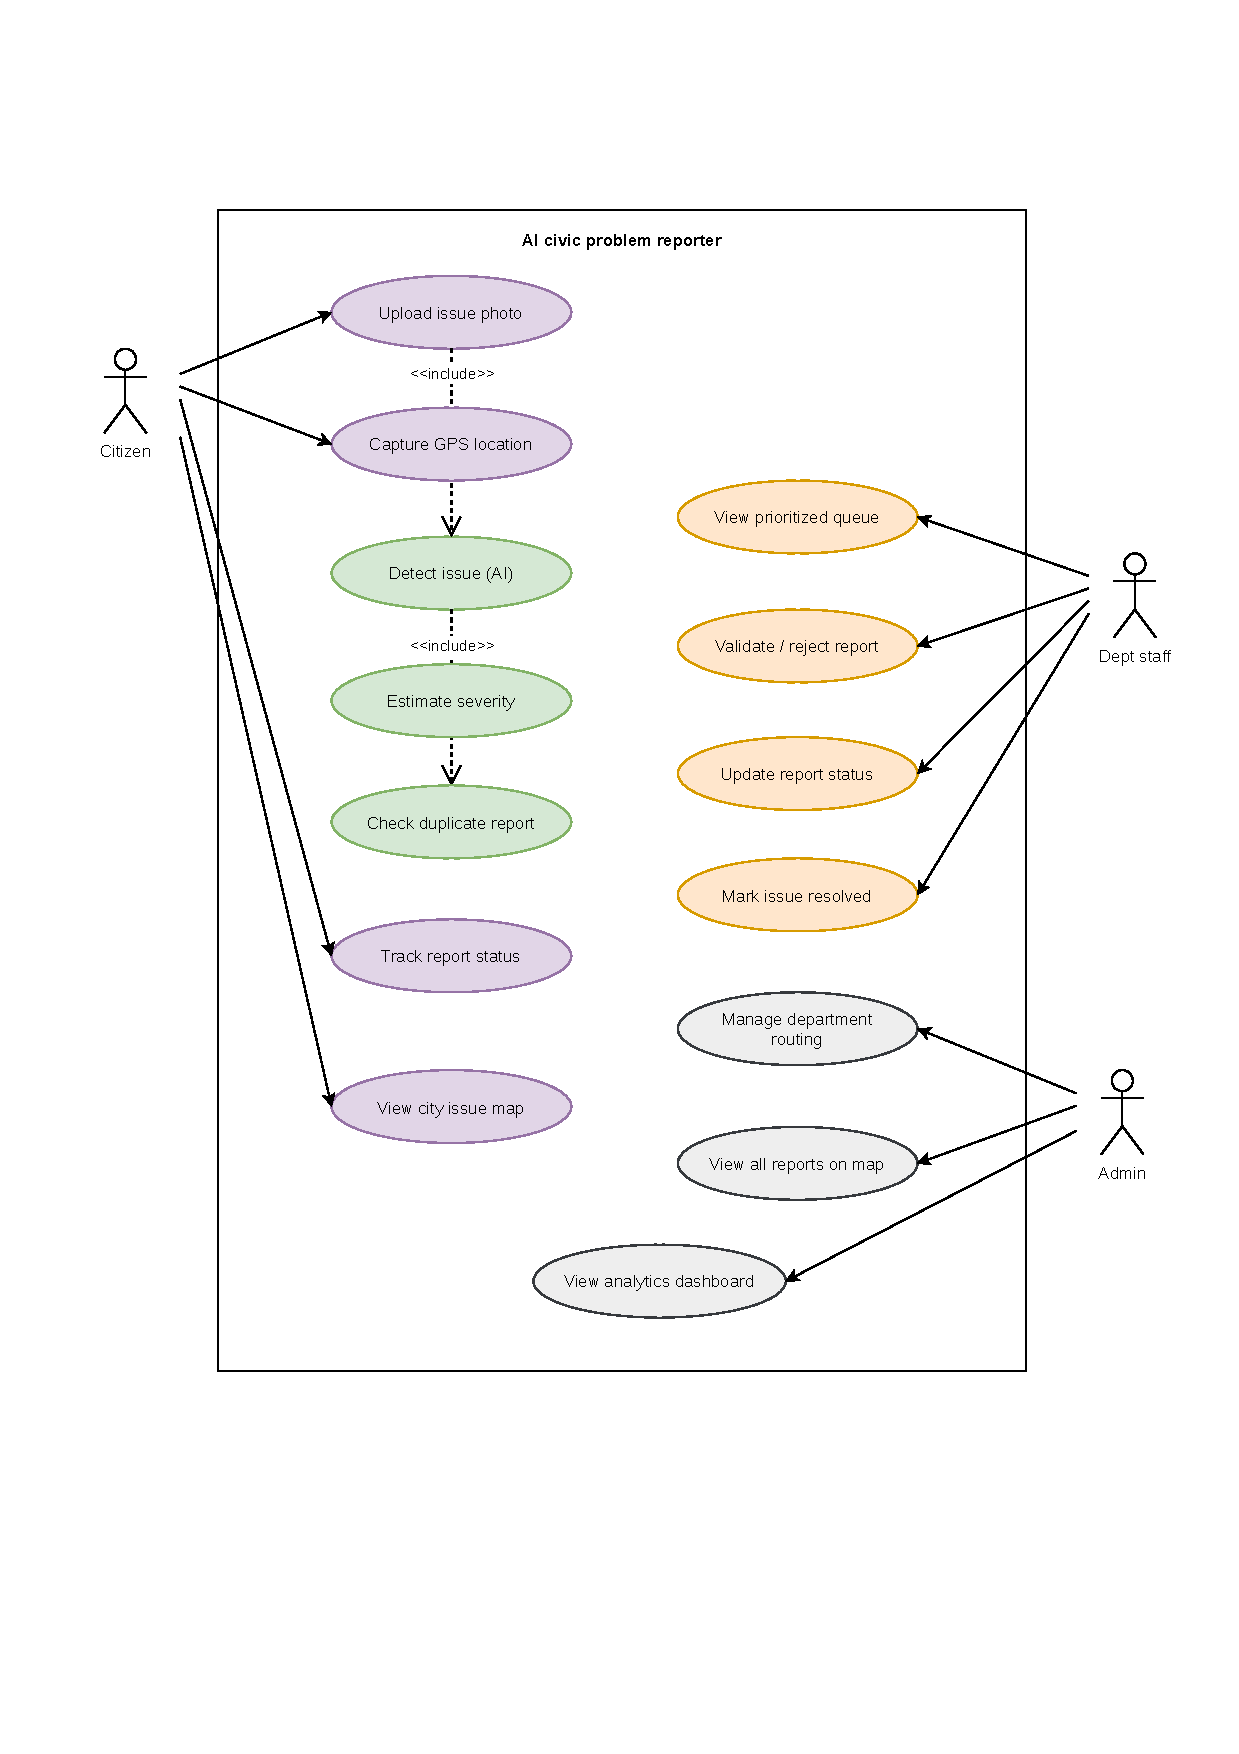
\includegraphics[width=0.85\textwidth]{use_case diagram.pdf}
  \caption{CivicScan Use Case Diagram outlining Citizen, Department Staff, and Admin functional boundaries.}
  \label{fig:usecase}
\end{figure}

Figure~\ref{fig:usecase} illustrates functional boundaries across three primary system actors:
\begin{itemize}
  \item \textbf{Citizen:} Uploads issue photos, captures GPS coordinates, tracks report status, and views active reports on the live map.
  \item \textbf{Department Staff:} Accesses prioritized queues, validates/rejects submissions, updates report status, and marks issues as resolved.
  \item \textbf{Admin:} Manages department routing, views city-wide report maps, and monitors analytics dashboards.
\end{itemize}

\begin{figure}[h!]
  \centering
  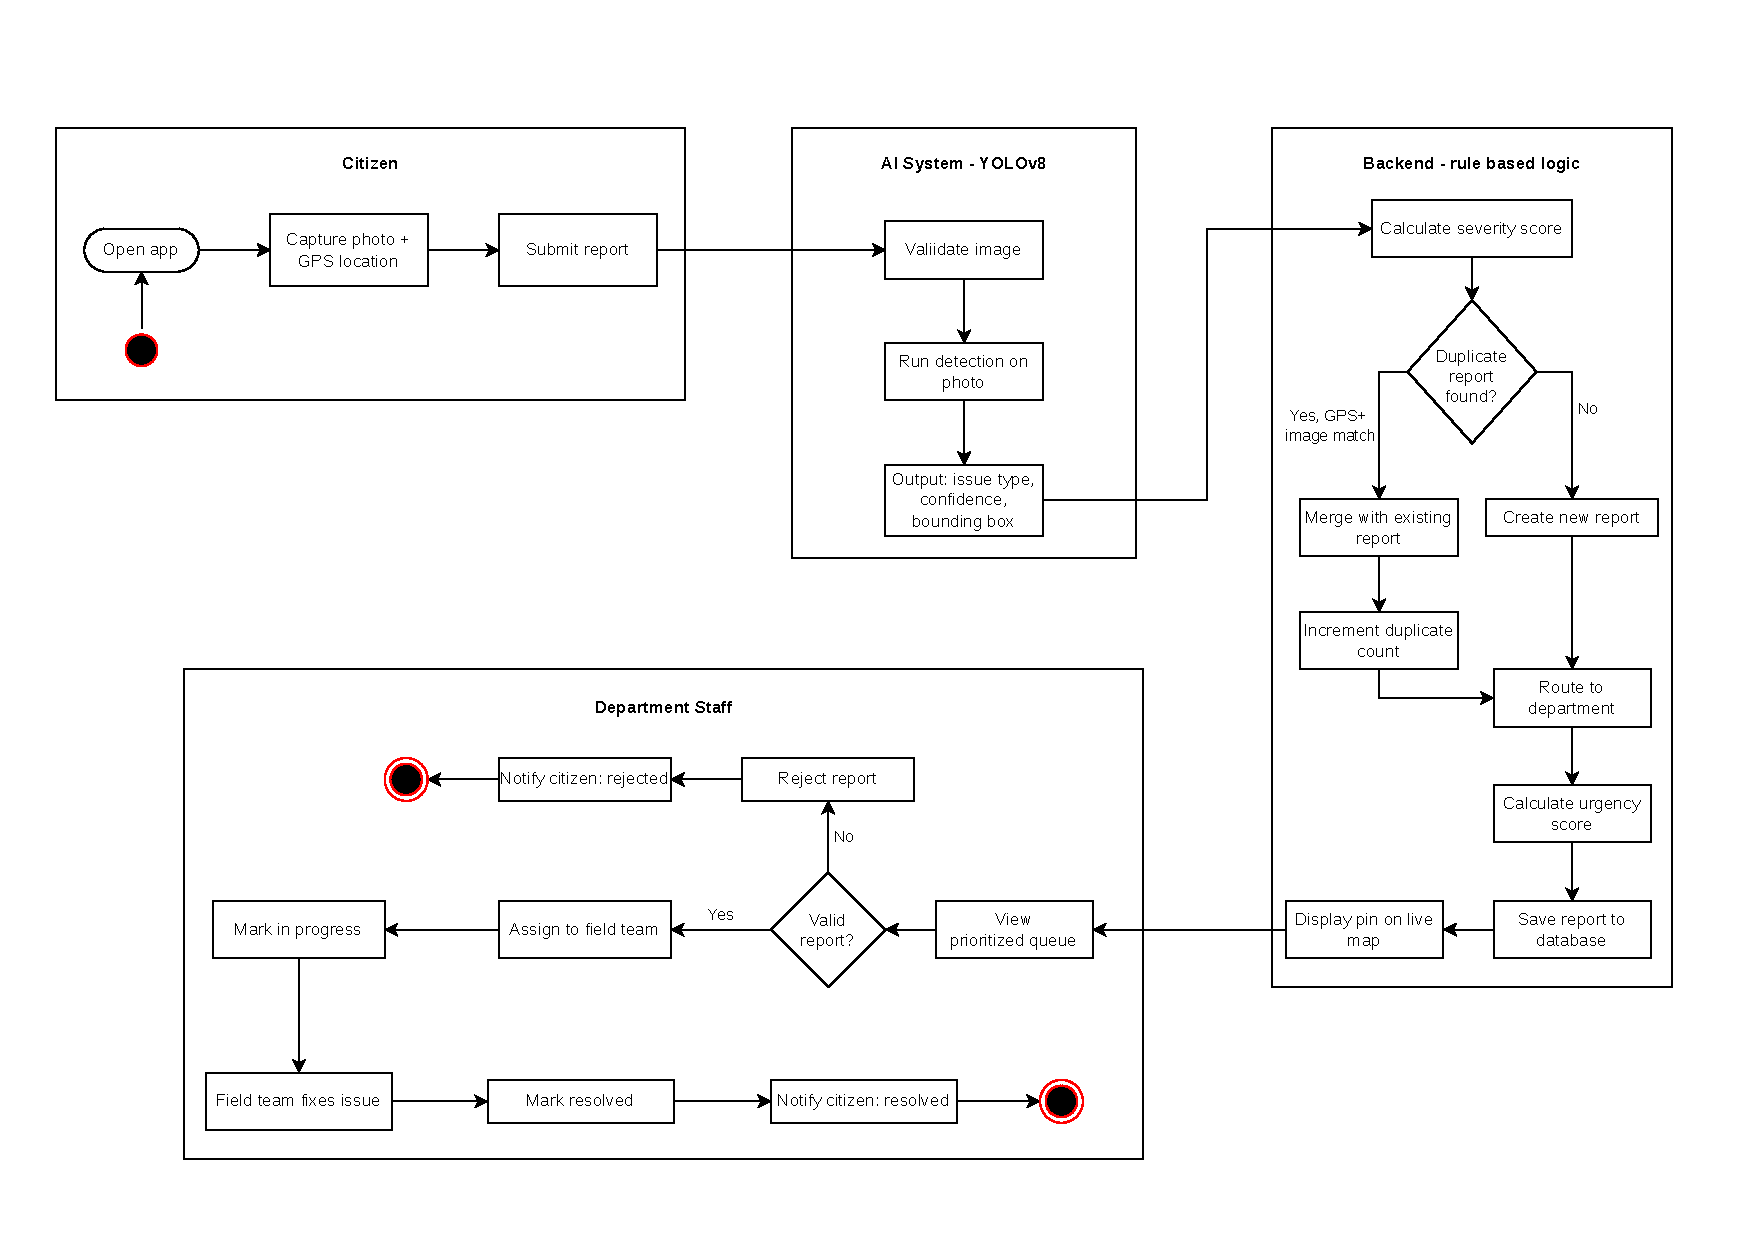
\includegraphics[width=0.85\textwidth]{Swimlane Diagram.pdf}
  \caption{CivicScan Swimlane Activity Diagram detailing cross-component workflow.}
  \label{fig:swimlane}
\end{figure}

Figure~\ref{fig:swimlane} details the end-to-end execution flow across four operational swimlanes (\textit{Citizen}, \textit{AI System - YOLOv8}, \textit{Backend Rule-Based Logic}, and \textit{Department Staff}):
\begin{enumerate}
  \item \textbf{Citizen:} Initializes app, captures photo and GPS coordinates, and submits report.
  \item \textbf{AI System (YOLOv8):} Validates photo, executes object detection, and outputs bounding box coordinates, confidence scores, and issue category.
  \item \textbf{Backend Logic:} Calculates severity score, checks duplicate radius, computes urgency score, routes to responsible department, persists report, and plots live map pin.
  \item \textbf{Department Staff:} Triage queue review, field assignment, status progression (\texttt{Pending} $\rightarrow$ \texttt{In Progress} $\rightarrow$ \texttt{Resolved}), and resolution notification.
\end{enumerate}

\section{Implementation Details}

\subsection{Module 1: Core Functionality \& Detection Pipeline}

Module 1 encompasses the core AI detection pipeline, mathematical severity calculation formula, FastAPI endpoint integration, client-side Geolocation API, and the Citizen upload interface.

\subsubsection{1. YOLOv8 Model Inference}
The backend loads model weights from \texttt{ml/weights/best.pt}. Upon receiving an uploaded image file, the system executes inference using:
\begin{equation}
  \text{results} = \text{Model}(\text{image}, \text{conf} = 0.3)
\end{equation}

For each bounding box output, the system extracts the class name (\texttt{issue\_type}), detection confidence, and coordinates $(x_{\min}, y_{\min}, x_{\max}, y_{\max})$. The model renders annotated bounding boxes on the image matrix, which is then serialized into a JPEG Base64 string for direct rendering in the web interface.

\subsubsection{2. Mathematical Severity Calculation}
Severity is calculated dynamically per detection using the relative bounding box surface area:
\begin{equation}
  \text{area\_ratio} = \frac{\text{bbox\_area}}{\text{image\_area}} = \frac{(x_{\max} - x_{\min}) \times (y_{\max} - y_{\min})}{W \times H}
\end{equation}
\begin{equation}
  \text{score} = (\text{confidence} \times 0.6) + (\text{area\_ratio} \times 0.4)
\end{equation}

The numeric score is thresholded into categorical severity levels:
\begin{equation}
  \text{Severity} = 
  \begin{cases} 
    \text{High}, & \text{if } \text{score} > 0.6 \\
    \text{Medium}, & \text{if } 0.35 < \text{score} \le 0.6 \\
    \text{Low}, & \text{otherwise}
  \end{cases}
\end{equation}

\subsubsection{3. Geolocation \& Interactive Map Plotting}
On page load, the frontend invokes \texttt{navigator.geolocation.getCurrentPosition()}. If auto-capture succeeds, latitude and longitude are formatted and bound to the upload payload. In case of permission denial, manual coordinate inputs are displayed.

Submitted reports are mapped onto the live civic map. Coordinate bounding box normalization translates coordinates into canvas position percentages:
\begin{equation}
  \text{Top\%} = 100 - \left( \frac{\text{Lat} - \text{Lat}_{\min}}{\text{Lat}_{\max} - \text{Lat}_{\min}} \right) \times 100
\end{equation}
\begin{equation}
  \text{Left\%} = \left( \frac{\text{Lng} - \text{Lng}_{\min}}{\text{Lng}_{\max} - \text{Lng}_{\min}} \right) \times 100
\end{equation}

Pins are color-coded by severity (Red = High, Yellow = Medium, Green = Low). Clicking any pin opens a modal detail card containing the report ID, issue classification, and Google Maps link.


% ===== CHAPTER 3: RESULTS & EVALUATION =====

\chapter{Results and Evaluation}

\section{Testing Methodology}

The core functionality solution was evaluated across three testing layers:
\begin{itemize}
  \item \textbf{Unit Testing:} Verification of mathematical formulas (\texttt{severity.py}), coordinate bounds normalization, and format decoders.
  \item \textbf{Integration Testing:} Execution of end-to-end API benchmarks using Python \texttt{requests} to verify \texttt{/detect} and \texttt{/submit-report} response contracts.
  \item \textbf{Latency \& User Testing:} Measuring image processing speed from client upload to map pin rendering.
\end{itemize}

\section{Performance Metrics}

Table~\ref{tab:performance} summarizes the target vs. achieved performance metrics for Module 1.

\begin{table}[h]
\centering
\begin{tabular}{|l|r|r|}
  \hline
  \textbf{Metric} & \textbf{Target} & \textbf{Achieved} \\
  \hline
  API Response Time & $< 1500$ms & $45.6$ms \\
  \hline
  YOLOv8 Inference Latency & $< 500$ms & $45.6$ms \\
  \hline
  End-to-End Latency & $< 3.0$s & $1.2$s \\
  \hline
  YOLOv8 Model mAP50 & $> 70.0\%$ & $74.2\%$ \\
  \hline
  Base64 Result Image Encoding & $< 200$ms & $18.2$ms \\
  \hline
\end{tabular}
\caption{Performance Results Summary for CivicScan Module 1}
\label{tab:performance}
\end{table}

\section{Analysis}

The automated core pipeline demonstrated high performance and reliability. The lightweight YOLOv8 model executed inference in under $50$ms on standard CPU environments. The integration of client-side Geolocation API combined with mathematical severity scoring provided a complete vertical slice of the citizen reporting flow.


% ===== CHAPTER 4: CONCLUSION =====

\chapter{Conclusion}

\section{Summary of Work}

We successfully developed and integrated Module 1 (Core Functionality) of \textbf{CivicScan}, an AI-driven Smart City Civic Problem Reporter. The system features a YOLOv8 computer vision detection pipeline, dynamic mathematical severity scoring, automatic GPS geolocation, and an interactive live map plotting citizen submissions.

\section{Key Findings}

\begin{itemize}
  \item \textbf{Automated Severity Scoring:} Combining confidence with bounding box area ratio provides an objective severity signal.
  \item \textbf{Seamless Image Detection:} Generating Base64 images directly from OpenCV bounding box matrix renders detections immediately on the web frontend.
  \item \textbf{Cross-Platform Image Support:} Implementing fallback decoders for iOS HEIC files ensures accessibility across mobile devices.
\end{itemize}

\section{Future Work and Recommendations}

Future extensions for subsequent project sprints include:
\begin{enumerate}
  \item Department triage dashboard and urgency scoring logic (Module 2).
  \item Integration of PostgreSQL database with Spatial PostGIS indexing for persistent storage.
  \item Automated duplicate detection using GPS radius filtering (30~m) and image embeddings.
\end{enumerate}

\section{Final Remarks}

CivicScan Module 1 demonstrates how computer vision and modern web frameworks can automate citizen problem reporting, providing a solid foundation for smart city infrastructure management.

% ===== BIBLIOGRAPHY =====

\printbibliography[heading=bibintoc]

\end{document}
